\section{Witnesses}


\noindent
In the pre-modern era, the \VSS\ has been transmitted exclusively in multiple-text manuscripts that were produced in Nepal. Even when a
manuscript of the \VSS\ seems to be a single-text MS, 
chances are high that it originally belonged to a multiple-text
manuscript.%
	\footnote{\label{noteonKolkataMs}As I remarked elsewhere 
	(\mycitep{KissVolume2021}{185, n.~9}):
	`Asiatic Society (Calcutta), Manuscript G 4076, cat. no. 4083, 
	may seem to be an independent manuscript of the 
	\textit{Vṛṣasārasaṃgraha}, but as De Simini has already 
	remarked (2016b, 240 n. 19),  % [= \mycite{DeSiminiMSSFromNepal2016}],
	it is probably from a multiple text manuscript. In fact, from what
	can be gathered from its description in
	\mycitep{SastriCatalogue5}{716ff},
	it seems likely that this manuscript was
	originally part of manuscript Asiatic Society (Calcutta) G 3852, cat.\
	no.\ 4085. See for example the folio numbering in these two 
	manuscripts: ASC G 3852 contains 210 folios, 
	and ASC G 4076 starts on folio 210.'}
In the manuscript descriptions below, in addition to some general
remarks, I will mainly focus on information relevant to the \VSS. For
much more detail on the overall features of these manuscripts, see 
\mycite{DeSiminiMSSFromNepal2016}, \mycite{BisschopUniversal}, 
\mycite{SaivaUtopia}, \mycite{SDhS10_ed},  
and the catalogues I mention
at some of the individual manuscript.%
		\footnote{I owe thanks to Florinda De Simini for 
			sharing with me most of the manuscripts listed here, to
  			Kengo Harimoto and Gudrun Melzer (Munich) for 
  			providing photos of the  Munich MS, and to 
  			Nirajan Kafle for sharing a digital 
  			copy of the Paris MS with me.}

In recently published and forthcoming critical editions of and articles
on the Śivadharma corpus,%
		 \footnote{\mycite{BisschopUniversal}, 
						\mycite{SaivaUtopia}, and \mycite{SDhS10_ed}.}
the sigla of the manuscripts used are made up of 
a letter signifying the script (e.g.~`N' for
Nepālākṣara/Newari), a superscript letter for the current location where
the manuscript is deposited (e.g.~`C' for Cambridge), 
and two (sometimes only one or even three) subscript 
digits echoing the last digit(s), if any, of the reference 
number of the manuscript in the 
library where it is located or, in the case of NGMPP reel 
numbers, the last two digits of the first part of the reel number.%
			\footnote{For details of this system and for the underlying reasons, see 
								\mycitep{BisschopUniversal}{50--51}.}
Since in the case of the \VSS\ all the 
manuscripts I utilised are written in
some variant of the Nepālākṣara script,%
		\footnote{I have not used NGMCP B 219/3 
		NAK 4/2537 (paper, Maithilī script), and \msL\
		(paper, Devanāgarī script, see below).} 
in this publication I omit the first letter, 
making the letter for the current location non-superscript. 
This helps keeping the apparatus readable. 
In the manuscript descriptions below, I give this 
omitted and implied `N' in brackets as a reminder.

Note that here I mention not only those MSS that
have been collated for the whole of, or parts of,
the critical edition, but also some that were candidates
for the task but later were dismissed.		

%\section{How to describe a MS?}\label{how-to-describe-a-ms}

%In general these categories should be included: - {[}X{]} Siglum - {[} {]} Location where it is deposited - {[} {]} Ms no. - {[} {]} How much do I use it? - {[} {]} Catalogued by and where and under what no., with what title - {[} {]} what does the catalogue says - {[} {]} Physical: - {[} {]} material - {[} {]} dimensions - {[} {]} no of folios - {[} {]} condition - {[} {]} format, binding - {[} {]} Text - {[} {]} script - {[} {]} contains these texts - {[} {]} complete - {[} {]} language (implied) - {[} {]} MTM? - {[} {]} foliation - {[} {]} hands - {[} {]} initial rubric, incipit, explicit, final rubric (in edition) - {[} {]} colophons (in edition) - {[} {]} dating - {[} {]} description in detail, remarks


\medskip
\label{mss_descr}
\subsection{Cambridge manuscripts}

\msdescr{(N)\msCa}{nc94}
Cambridge University Library, Add. 1694.1. This MS has been 
fully collated for chapters 1--12 of the critical edition in this volume. 
See a detailed description of this manuscript in the 
CUDL online catalogue.\footnote{https://cudl.lib.cam.ac.uk/view/MS-ADD-01694-00001/382}
According to this catalogue, the date of creation of this manuscript 
is the 12th century, and its dimensions are 5~×~ca.\thinspace 53.5 cm. 
The script is Nepālākṣara. It is a palm-leaf multiple-text manuscript containing 258
folios and transmitting eight texts: 
1)~\SDhS,
2)~\SDhU,
3)~\SDhSangr,
4)~\Ums,
5)~\Uums, 
6)~\Vss,
7)~\DharmP,
8)~\SivaUp.

The \VSS\ occupies 45 folios: it starts on \fol193v. 
The recto side, online image no.\thinspace381, is an empty folio side. 
The text ends on \fol239r (online image no.\thinspace473). 
The text of the \VSS\ is transmitted fully,
without any folios or major sections of the text missing. The leaves
transmitting the \VSS\ are well-preserved. Some folio sides are faded and
most folios are somewhat damaged on the right side, 
sometimes at other parts, and it seems from the images 
that some opaque-looking tape has been applied to protect these damaged sections. 
In my critical edition the broken off, completely lost, 
\emph{akṣara}s are represented by \lac,
the illegible \emph{akṣara}s under the tape by \lk\ (`illegible'). The
quality of the readings of this manuscript is one of the best among
the available witnesses, comparable only to \msNa\ and \msParis, 
making it one of the most important sources for the \VSS.


\msdescr{(N)\msCb}{nc45}
Cambridge University Library, Add. 1645. This MS has been fully
collated for chapters 1--12 of the critical edition in this volume. 
See a detailed description of this manuscript in the CUDL online catalogue.\footnote{https://cudl.lib.cam.ac.uk/view/MS-ADD-01645/404}
According to this catalogue, its dimensions are 
4.4~×~61.7~cm. The manu\-script is dated to (Nepāla) `\emph{samvat} 259
\emph{śrāvaṇa śukla dvādaśiyā di} \textless{} \emph{trayodaśyām},'
which converts to July 10/11 Monday/Tuesday, 1139 \CE.%
		 \footnote{\Fol247r line 6. The CUDL website transcribes this
		  colophon as: \skt{saṃvat} 259 
		  \skt{śrāvaṇaśukladvādaśi{\rm[}pyaḍi} 8 
		  \skt{trayodaśyāṃ} (retrived 8 Dec 2021). 
		  The element \skt{dvādaśipyaḍi} could be read as
		  \skt{dvādaśiyā di}, perhaps a mistake for
		   \skt{dvādaśyāṃ}
		  \skt{di} (\skt{di} for a misplaced \skt{diva/divā}?), and the
		  symbol that does look like a figure `8' of a slightly later period
		  than the manuscript itself (resembling the mathematical symbol
		  \textless{}) might also be a \skt{kākapada}. 
		  Alternatively, one could understand \skt{yā} as a Newar genitive marker,
		  \skt{dvādaśi-yā di} meaning `the day of the twelfth.'
		  Another faint
		  \skt{kākapada} is perhaps to be seen under \skt{daśi},
		  therefore it is possible that the scribe's intention was to delete 	
		  \skt{dvādaśi} and correct it to \skt{trayodaśyām}, 
		  and then the date becomes 11th of July.
		  Kengo Harimoto 
		  has suggested that the unclear element
		  (\skt{yādi/pyaḍi}) is in fact \skt{ghaṭi}, 
		  and after comparing these two syllables to other instances of
		  \skt{gha} and \skt{ṭa}, one cannot but agree. 
		  In this case this should be an indication of the
		  exact time (Skt. \skt{ghaṭi/ghaṭikā}, Newar \skt{ghaṭi}) 
		  the scribe finished copying the text. It is still not clear
		  if we should take \skt{dvādaśi} or \skt{trayodaśyām} 
		  as the date. For help on the conversion of the date and 
		  for a detailed discussion on the colophon I am indebted
		  to Kengo Harimoto.} 
The script is Nepālā\-kṣara. It is a palm-leaf multiple-text 
manuscript containing 247 folios. Eight texts are transmitted 
in this manuscript: 
1)~\SDhS,
2)~\SDhU,
3)~\SDhSangr,
4)~\SivaUp,
5)~\Ums,
6)~\Uums, 
7)~\Vss,
8)~\DharmP.


The \VSS\ occupies 37 folios plus one folio side: it starts on \fol201v
line 4 (online image no.\thinspace 404), 
and it ends on \fol238v line 3 (online image
no.\thinspace 478). 
The readings of this manuscript seem to follow those of \msNa\
remarkably closely while transmitting the 
Śivadharmottara (as observed by De Simini and Harimoto).%
\footnote{Personal communication, 1 Dec 2021.} This
is more difficult to see in the case of the \VSS, 
but indeed, they seem closely related. 
%CHECK MORE on this


\msdescr{(N)\msCc}{nc02}
Cambridge University Library, Add.\thinspace 2102. 
All available folios of this MS have been collated for 
chapters 1--12 of the critical edition in this volume. 
See a detailed description of this manuscript 
in the CUDL online catalogue.%
	\footnote{https://cudl.lib.cam.ac.uk/view/MS-ADD-02102/181}
According to this catalogue, the date of creation is the 12th
century, and the dimensions of the manuscript are 
4.8~×~ca.\thinspace 52.5~cm. 
The script is Nepālākṣara. It is a palm-leaf multiple-text manuscript
containing 96 folios. Six texts are transmitted in this manuscript: 
1)~\SDhU,
2)~\SDhSangr,
3)~\Ums,
4)~\SivaUp,
5)~\Vss,
6)~\DharmP\ (only \fol322v). 
Note that the \SDhU\ starts on \fol51r, thus the part that most probably contained the \SDhS\ is lost.

The \VSS\ starts on \fol267r line 1 
(online image no.\thinspace181). 
The online description labels this image as \fol237r. 
This first folio in fact has no visible foliation.
The previous text, the \SivaUp,
ended on \fol236v, with pāda b of verse 7.122,%
 		\footnote{Image no.\thinspace180, 
                  \SivaUp\ 7.122: \skt{yauvanasthā gṛhasthāś ca}
                  {[}\skt{prāsā}{]}\skt{dasthāś ca ye nṛpāḥ}.}
which is not the end of the \SivaUp: 
about eighteen verses, probably transmitted 
in one single folio, are lost.
This means that, if the foliation and the order of the folios
are presented correctly, and if the portion containing
the \VSS\ indeed belongs to the same manuscript, 
folios 237--266, i.e.\ thirty folios, are missing. 
They must have transmitted the \Uums, 
which takes up twenty-three folios in \msCa, and twenty folios in \msCb.
Thus this MS did most probably transmit all eight texts of the
Śivadharma corpus.%
	\footnote{Compare with the claim of the online catalogue:
		``The present manuscript probably contained seven texts.''}	

This first folio of the \VSS\ is in a hand which is different from the
rest of the manuscript, but the hand changes back in the next folio.\label{msCcfirstfolio}%
	\footnote{Cf.~the metadata on the CUDL site: 
	`1 folio of the same dimensions is a modern supply for the 
	beginning of the \skt{Vṛṣasārasaṃgraha}.' A hardly readable 
	note in pencil to the same effect is visible at the
    top of the first folio side (\fol267r, `mode\ldots\ldots 
    supply beg of Vṛṣasāra-saṃgr.'). I am not sure how `modern'   
    this supplement is, but it seems indeed likely that a lost 
    first folio was supplemented
    with a later copy. To match the end of this new copy with the
   beginning of the next, older, folio, a scribe more or less erased   
   the beginning of the first line in the old folio, 
   rather than the last line
   of the younger folio. 
   This slightly illogical decision may mean that the younger
   copy was not tailor-made for the old portion, 
   but rather that it was
   taken from a younger manuscript which was 
   perhaps considered more legible. 
   Otherwise it would have been more practical to stop copying
   the first folio at the point where the next begins.
   See some more detail on this folio on
    p.~\pageref{msCcfirstfoliokakapada} below.}




In this multiple-text manuscript, the \VSS\ is trasmitted in an incomplete
form, that is to say, a number of folios are missing (most notably
chapters 15--17). The first partially visible folio number is in image
184: the numeral characters 200+60 are visible (268v, according to the
CUDL online catalogue). In image 186, the folio number 269 is clearly
visible (\fol269v). In folio 270v, the continuous text is broken at verse
2.21c (\skt{kāmarū°}), \fols271 and 272 are missing, and the text
resumes on \fol273r with verse 3.30b ({[}\skt{ahiṃsā
pa}{]}\skt{ramaṃ} \skt{sukham}). Folio 291 is missing (verses
12.87cd--12.113). In folio 296v (image no. 234) the text breaks off
again at \skt{vātaśūlair upadrutā} | \skt{śukro} (verse 14.22b),%
        \footnote{Of course, my verse numbering in chapters 13--24 may change slightly
                  during the editing process.}
the next folio being 306r (starting with \skt{carmatāś ca dvijasundarīṣu},
verse 18.27b; nine folios and chapters 15--17 are completely
missing).

Again, there are two missing folios after \skt{bandhus sarvva°} in
verse 18.47c in \fol306v. The text resumes in \fol309r (image 237)
with \skt{°ṇeṣu ca sarvveṣu vidvān sreṣṭha sa ucyate} (verse 19.52cd). Another folio is missing between \skt{iṣṭāniṣṭadvaya°} (verse
20.22, \fol309v) and \skt{snāyu majjā sirā tathā} (verse 20.51d, \fol311r). The \VSS\ ends on \fol322v (image no.\thinspace262) with the
concluding colophon \skt{vṛṣasārasaṅgraha samāpta iti}. 
This folio also contains the beginning of the \skt{Dharmaputrikā}, 
but this multiple-text manuscript contains no more folios.

In the apparatus, the siglum \mssCaCbCc\ signifies all three Cambridge 
MSS described above.

\medskip
\subsection{Kathmandu palm-leaf manuscripts}
\msdescr{(N)\msNa}{nk82}
NGMPP A 1082/3, NAK 3/393. This MS has been fully 
collated for chapters 1--12 of the critical edition in this volume. 
See a brief description of this MS in
the NGMCP online catalogue.%
	\footnote{https://catalogue.ngmcp.uni-hamburg.de/receive/aaingmcp\_ngmcpdocument\_00098499}
According to this catalogue, the dimensions of the 
manuscript are 55.6 × 5.5 cm. 
It is dated to Nepāla Samvat 189 (1068--69 \CE).%
	\footnote{See \fol12r line 2 of the 
	\DharmP\ in this MS: 
	\emph{navottarāsītiyute sate bde āsāḍhaśuklasya
  tithau tṛtīye}, translated by \mycitep{DeSiminiMSSFromNepal2016}{252 n.\thinspace 49} as: 
  `in {[}the year{]} 189, in the 3rd lunar day of the bright {[}fortnight{]}
  of {[}the month{]} Āṣāḍha.' She adds that the date is verified in
  Petech 1984, 46 as May 24, 1069 \CE.} The script is Nepālākṣara. It is
a palm-leaf multiple-text manuscript containing 274 folios. Eight texts
are transmitted in this manuscript: 
1)~\SDhS,
2)~\SDhU,
3)~\SDhSangr,
4)~\Ums,
5)~\SivaUp,
6)~\Vss,
7)~\DharmP,
8)~\Uums.

As for each text in this collection, the foliation for the
\VSS\ restarts from \fol1v (\fol1r is a cover) and the text
spans \fols1v--46r. This is a beautifully written and well-preserved
manuscript which gives very useful readings and has proved to be
essential for the reconstruction of the \VSS.%
	\footnote{See a similar evaluation in
					\mycitep{BisschopUniversal}{56}.}


\msdescr{(N)\msNb}{nk10}
NGMPP A 10/5, NAK 1/1261. This MS has been fully collated 
for chapters 1--12 of the critical edition in this volume. 
See a brief description of this MS in
the NGMCP online catalogue.\footnote{https://catalogue.ngmcp.uni-hamburg.de/receive/aaingmcp\_ngmcpdocument\_00085264}
According to this catalogue, the dimensions of the manuscript are 55 x
5.5 cm. It is an undated palm-leaf multiple-text manuscript containing 74
folios. Four texts are transmitted in this manuscript: 
1)~\SDhU,
2)~\Ums,
3)~\SivaUp,
4)~\Vss.

Some folios feature drawings. 
A great number of the leaves that 
transmit the \VSS\ are damaged and, 
at least judging from the microfilm images, 
faded and slightly disordered. The folio numbers are
rarely visible. The \VSS\ starts on exp.\thinspace 44 
(upper leaf, no folio number is visible here). 
The text continues on the lower leaf and then on the upper
leaf on exp.\thinspace43 (going backwards, so to say) 
up to 1.60 (\skt{viṃśakoṭiṣu gulmeṣu ūrdhva°}). 
Verses 1.60d--2.22 seem to be missing. The lower leaf on
exp.\thinspace43 contains verses 2.23--2.39. 
The single leaf in exp.\thinspace42 contains
verses 2.40--3.16a. Exp.\thinspace41 contains a single leaf of the
\skt{Umāmaheśvarasaṃvāda}, ending in a colophon for its chapter
twenty-two, and still going backwards, the preceding folios continue
transmitting the 
\Ums. 
Exploring the presence of
the \VSS\ in this manuscript further, 
one should look at the expositions
after no.\thinspace44. Exp.\thinspace45 contains the end of the
\SivaUp. The
single leaf on exp.\thinspace46 
is almost illegible but most probably contains a
fragment of the 
\titleface{Gautama\-dharma\-sūtra}\index{Gautamadharmasutra@\titleface{Gautamadharmasūtra}}. 
The second line just above
the string hole on the left reads \skt{\ldots{} vīrud vanaspatīnāṃ ca
puṣpāṇi svavad} \skt{ādadīte\ldots{}}, which is a fragment of
\titleface{Gautama\-dharma\-sūtra}\index{Gautamadharmasutra@\titleface{Gautamadharmasūtra}}
2.3.25 (12.28). 
The remaining parts of the \VSS\
are to be found on exp.\thinspace47ff. 
The upper leaf on exp.\thinspace47 continues with
\VSS\ 3.16b--36ab, while the lower leaf contains a text that I have not
been able to identify. The lower leaf in exp.\thinspace48 transmits
3.36cd--4.11ab, the upper one 4.11b--30a. The lower leaf in 
exp.\thinspace49 contains 4.30ab--47ab, 
the upper one 47d--68a, and so on so forth. Thus
when reading the text from these images, after exp.\thinspace48, 
one has to start with the lower leaf and continue with the upper one.


\msdescr{(N)\msNc}{nk7}
NGMPP B 7/3 = A 1082/2, NAK 1/1075. This MS has been 
fully collated for chapters 1--12 of
the critical edition in this volume. See a brief description of this MS
in the NGMCP online catalogue.\footnote{https://catalogue.ngmcp.uni-hamburg.de/receive/aaingmcp\_ngmcpdocument\_00062373}
According to this catalogue, the dimensions of the manuscript are 
58 × 6 cm. The script is Nepālākṣara. Dated to Nepāla Samvat 
290 (1169--70 \CE). It is a
palm-leaf multiple-text manuscript containing 289 folios. Eight texts
are transmitted in this manuscript: 
1)~\SDhS,
2)~\SDhU,
3)~\SDhSangr,
4)~\Ums,
5)~\SivaUp,
6)~\Vss,
7)~\Uums,
8)~\DharmP.
\Fols209v--264v contain the \VSS.

This is a nicely written manuscript, giving generally useful and
convincing readings. 


\msdescr{(N)\msNd}{nk3}
NGMPP A 3/3 (= A 1081/5), NAK 5-737. I have collated 
this MS only for verses 1.1--15ab to test it. 
See a brief description of this MS in the NGMCP online
catalogue.%
	\footnote{http://catalogue-old.ngmcp.uni-hamburg.de/mediawiki/index.php/A\_3-3\_Śivadharma} 
According to this catalogue, the dimensions of the manuscript are
58.5 x 5.5 cm. The script is Nepālākṣara and the MS is dated 
to Nepāla Samvat 321 (1200--01 \CE). It is a palm-leaf multiple-text manuscript containing 215 folios.
Eight texts are transmitted in this manuscript: 
1)~\SDhS,
2)~\SDhU,
3)~\SDhSangr\ (only a few folios are extant, e.g. \fols124 and 143), 
4)~\Ums,
5)~\SivaUp,
6)~\Uums,
7)~\Vss,
8)~\DharmP.

The \VSS\ starts in \fol227 (image no.\thinspace177) 
and seems to end after it begins transmitting chapter 23 
in \fol264 (image no.\thinspace 218), but the last image 
(no.\thinspace253) also contains a fraction of \VSS\ chapter 13.
The microfilm images are somewhat blurred and the 
readings do not seem promising.


\bigskip

\noindent
Other palm-leaf MSS preserved in Kathmandu, but not used for
this critical edition include the following:

NGMPP A 11/3, NAK 5--738% 
%Palm-leaf, dated to NS 516 (1395--96 CE), 253 folios. Contents: Śivadharmaśāstra (fols.~1v--43r); Śivadharmottara (fols.~4v--95r); Śivadharmasaṃgraha (fols.~96v--139v); Umāmaheśvarasaṃvāda (fols.~140v-- 171r); Śivopaniṣad (fols.~172v--189r); Uttarottaramahāsaṃvāda (fols.~190v-- 211v); Vṛṣasārasaṃgraha(fols.~212v--257v). For a description of this manuscript, also see the record in the NGMCP online catalogue: \textless{}
	\footnote{http://catalogue.ngmcp.uni-hamburg.de/wiki/A\_11- 3\_Śivadharmottara}%
---the microfilm images of the folios containing the \VSS\ are often blurred to an extent that makes them
difficult to use.


NGMPP C 25/1, Kesar Library 218---this multiple-text manuscript
preserves only a few disordered folios of the \VSS.
%Palm-leaf, 298 folios.
%Contents: Śivadharmaśāstra (fols.~1v--57r); Śivadharmottara (fols.57v--134v); Śivadharmasaṃgraha (fols.~135r--215v); Umāmaheśvarasaṃvāda (fols.~216v--255r); Śivopaniṣad (fols. 256v--278r); Umottara°/ Uttarottaramahāsaṃvāda (fols. 279v--299v¤); Vṛṣasārasaṃgraha (?¤--?¤); (?--?¤).

\bigskip

\subsection{Kathmandu paper manuscripts}

\msdescr{(N)\msPaperA}{msPaperAdesc}
NGMCP A 1341/6, NAK 4--93. Paper, 82 folios,
probably from the 17th century (see the
description of \msPaperC\ below). 
This MS contains two texts: 
\SDhSangr\ (\fols91r--135v) and 
\Vss\ (\fols204r--243v). Collated only for
chapters one and eight in this volume, 
but consulted often at problematic passages.
As already seen
from the folio numbers, this multiple-text
manuscript must have contained more than two
texts originally, most probably of the
Śivadharma corpus. 
The script of this MS seems extremely similar to that 
of \msPaperC, a MS dated to 1688 \CE\ (see below).
Thus it seems probable that this MS is also
from the 17th century.

\msPaperA\ is a good example to see how relatively
late witnesses, a paper MS, can be important. Its readings
are relatively independent of most palm-leaf MSS,
and seem to shed some light on what source(s) 
Naraharinath may have used because there
are a great number of instances where \Ed\ and \msPaperA\
(and \msPaperC, see below) 
read together against most other witnesses. E.g., \msCa, \msCb, \msCc, \msNa, \msNb, \msNc, \msNd, 
and \msM\ read \skt{bhāratasaṃhitām}, or a slightly
corrupt form of the same, in 1.2cd, while the two
paper MSS \msPaperA, and \msPaperC, 
and Naraharinath's \Ed\ read (a clearly wrong)
\skt{nāradasaṃhitām}. Similarly, in 1.17cd most
witnesses read \skt{vettum arhasi}, while 
\msPaperA, \msPaperC, and \Ed\ (and \msM!) read
\skt{vaktum arhasi}. In 1.44b, \msPaperA\ and
\Ed\ read \skt{mṛddhe}% 
		\footnote{\msPaperC\ reads a similar
					\skt{gṛdbhe}.}
instead of \skt{śṛṇu} and \skt{śṛṅge} 
in all other witnesses.
In some instances, the paper
MSS \msPaperA\ and \msPaperC\ give readings
that might be old or `original.' E.g., 20.40d is missing
in a great number of MSS (\msCa, \msCb, \msNa, \msNb),
\msNc\ gives (improvises?) a less than perfect 
\skt{tān nibodha dvijottamaḥ},%
		 \footnote{One would expect the vocative
		 				\skt{dvijottama}.}
while \msPaperA, \msPaperC, and \Ed\ give a similarly imperfect
\skt{vijñeyā ca manīṣibhiḥ}.%
		 \footnote{The correct sandhi would be
		 				\skt{vijñeyāś ca}.}
Sometimes these two paper MSS either alter
the text, or again, preserve older readings. 
E.g., in 16.34 \msPaperA, \msPaperC, and \Ed\
give \skt{bhagavān uvāca} against all other witnesses'
\skt{maheśvara uvāca}. After 12.30d (\skt{vipulaḥ punar abravīt}),
\msPaperA, \msPaperC, and again \Ed, insert
a somewhat unnecessary \skt{vipula uvāca}. These
and many other examples could prove that
Naraharinath used manuscripts that were close
to \msPaperA\ and \msPaperC,\label{narahari_paperms}
and some of the oddities in his edition originate in fact in 
actual readings rather than misreadings or
20th-century alterations.%
		\footnote{Compare this with 	
					\mycitep{SaivaUtopia}{58--59}, especially the
					following piece of information:
					`According to the information kindly
					provided by Diwakar Acharya (personal communication),
					it may have been based on a Devanāgarī manuscript 	
					from the time of Raṇa Bahādur Shah (1775--1806).'}

Another fascinating phenomenon in \msPaperA\ is
traces of editorial activity. There is a rather
peculiar \skt{kākapada}, or editorial sign to mark
omission, that could help us catch a perhaps
17-19th century editor red-handed while he is inspecting,
correcting, and sometimes altering the text, and 
also while he is consulting older palm-leaf MSS.
The sign can be spotted, e.g., in \msPaperA\
on top of a \skt{ku}, indicating that the syllable \skt{ru}, 
given in the top margin,
should be inserted there; 
doubled in the same MS to indicate a larger omission; 
in MS NGMPP C 57/5, another paper Śivadharma corpus
multiple-text MS, to indicate a alternative reading;
and in the much older palm-leaf MS, 
\msNa, to indicate a missing passage,
which is in fact to be found in at least two paper MSS 
(\msPaperA\ and \msPaperC) and in Naraharinath's
edition  (see Figure \ref{fig:kakapadas}).

\begin{figure}
\hspace{3em} 

\includegraphics[scale=.2]{images/mspaperA227rkakapadablurred.png}
\hfill

\includegraphics[scale=.2]{images/doublekakapada_msPaperA238r.png	}
\hfill

\includegraphics[scale=.4]{images/C57_5_kakapada7v.png}
\hfill
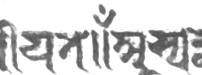
\includegraphics[scale=.5]{images/dottedkakapada01.png}
%
\includegraphics[scale=1]{images/dottedkakapada_small.png}
\hspace{3em}

\hspace{2em}
\msPaperA\ \fol229\recto
\hspace{1.5em}
\msPaperA\ \fol238\recto\
\hspace{.7em}
C 57/5 \fol7\verso\
\hspace{2.4em}
\msNa\ \fol45\verso
\hspace{2em}
\caption{\skt{Kākapada}s\label{fig:kakapadas}}
\end{figure}

Consulting \mycite{EinickeKorrektur}, 
a rich catalogue of editorial marks,
one gets the impression that this type 
of \cskt{kākapada}{kakapada}, which has a dot in it,
is not frequently seen. Two instances of such a 
 \cskt{kākapada}{kakapada} 
  occur in two NGMPP 
 \titleface{Viṣṇudharmaśāstra} MSS from 1661 and 1713 \CE,%
 		\footnote{MSS G 18/2 and B 218/2, 
 							\mycitep{EinickeKorrektur}{161--162 and
 										236}.}
one in the above mentioned Śivadharma MS 
NGMPP C 57/5 from 1826 \CE,%
		\footnote{\mycitep{EinickeKorrektur}{164 and 328}.} 
 and in a \titleface{Kālacakratantra} MS written 
 in old Bengali script from 1446 \CE, 
 which has (most probably much later) corrections
 in Nepālākṣara script.%
 					 \footnote{\mycitep{EinickeKorrektur}{65--66 and 328}.
 					 On p.~66, Einicke remarks: `Besonderheiten: 
 					 Korrekturen einzelner Zeichen in späterer 
 					 Newārī-Schrift am Rand'.}
 				 
It is difficult to escape the impression that
we are dealing with the same editor, whose
distinguishing mark is a \cskt{kākapada}{kakapada} 
with a dot. If indeed MS C 57/5 (1826 \CE) also bears
his hallmark, then he must have been a pundit from 
the 19th or 20th century. He seems to have performed
some rather detailed and focused editorial activities, and
must have had access to some of the old palm-leaf MSS.
One telling example for this is his marking the omission
in \msNa\ of two \skt{anuṣṭubh} verses on heavens after
\VSS\ 24.72 (see image on the right in Figure
\ref{fig:kakapadas}). 
As hinted at above, these verses, 
potentially later insertions, occur in the paper MSS
 \msPaperA\ and \msPaperC, and in Naraharinath.
To spot this, our anonymous editor had to
carefully compare the old palm-leaf MS with the 
17th-century paper MS.%
		\footnote{More on this in volume two.}
 				 
\label{msCcfirstfoliokakapada}
These observations also shed some light on
the origin of the first folio of \msCc, which is in 
a hand that looks later than that in the rest of that MS.%
		\footnote{See p.~\pageref{msCcfirstfolio}.}			 
Most old palm-leaf MSS start with \skt{karmahetuḥ śarīrasya}
etc.\ at \VSS\ 1.14ab , while the two 
paper MSS \msPaperA\ and \msPaperC, 
and Naraharinath read \skt{anarthayajña uvāca || karmahetuḥ śarīrasya}. The only palm-leaf MS that reads with 
the paper MSS is \msCc, on its only folio that is
written in a later hand. This at least tells us that
the supplied first folio in \msCc\ comes from a
source that is closer to the paper MSS than to the
old palm-leaf MSS, and it could also be another piece
of evidence for editorial activity by someone who
carefully examined these sources, and in addition,
introduced fresh contamination. \label{vipulauvaca}For this kind
of easy-to-spot contamination, a good example is
the insertion of the somewhat unnecessary
\skt{vipula uvāca} in palm-leaf NS \msCc\ after 12.30,
inspired by paper MS \msPaperA, 
and/or \msPaperC\ (see Figure \ref{fig:vipulauvaca}).
\begin{figure} 
\hfill
\includegraphics[scale=.1]{images/vipulauvaca_mscc_12.31monochrome.png}
\hfill
\includegraphics[scale=.2]{images/vipulauvaca_papermsa_12.31.png}
\hfill
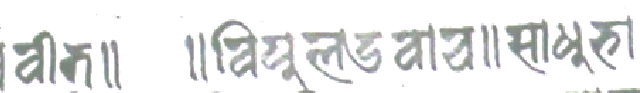
\includegraphics[scale=.2]{images/vipulauvaca_msPaperC223v.png}
\hfill

\hspace{2em}
\msCc\ \fol288\verso
\hspace{5em}
\msPaperA\ \fol219\recto
\hspace{6em}
\msPaperC\ \fol223\verso
\hspace{3em}
\caption{Insertion of \skt{vipula uvāca} in \msCc\label{fig:vipulauvaca}}
\end{figure}
Note the tiny \skt{kākapada} with the dot
on the palm-leaf on the left and
the insertion in a different hand in the margin below.
It seems probable that our anonymous editor
went through some paper MSS and noted differences
in the palm-leaf MS \msCc\ (and in \msNa, see Figure
\ref{fig:kakapadas}). 

\medskip

\msdescr{(N)\msPaperC}{msPaperC}
NGMCP C107/7, NAK 9/537. Paper. Size: 
37.1~×~10.8 cm. 174 folios. This MS is
dated to NS 809 (1688--89 \CE),%
		\footnote{\raisebox{-.8em}{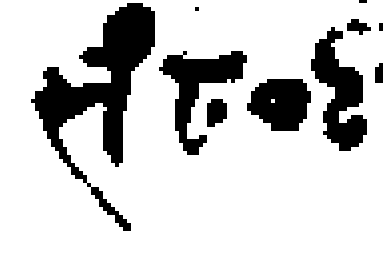
\includegraphics[scale=.1]{images/msPaperCf262vDating02.png}} (\fol262v). 
		De Simini reads NS 803
		(\citeyear{DeSiminiMSSFromNepal2016}, 253 n.~51).
		I prefer reading NS 809. }
Folios 1--88 are missing. These must have contained the \SDhS\ and the \SDhU.%
			\footnote{Cf. 
				\mycitep{DeSiminiMSSFromNepal2016}{252 n.~48}. 
				See also an unfinished table of contents on \fol262r,
				which confirms that at least the \SDhS\ was part 
				of this bundle: \skt{|| asyānukramaḥ || 
				prathama śivadharmo nāma}.}
The MS thus contains only six texts:
1)~\SDhSangr\ \fols89r--133v,
2)~\Ums\ \fols134r--163v,
3)~\SivaUp\ \fols164r--181r,
4)~\Uums\ \fols182r--206v,
5)~\Vss\ \fols207r--251v, % img 8345
6)~\DharmP\ \fols252r--262v. 

The script of this 17th-century MS seems 
extremely similar to that of \msPaperA, 
therefore the latter can also be
dated to the 17th century. USE IT? \CHECK



\medskip
\subsection{Munich manuscript}

\msdescr{\msM}{munichMS}
This MS is preserved at the Ludwig Maximilian University
in\linebreak \mbox{Munich}, Germany.%
			\footnote{\mycitep{HarimotoMunichMS}{596}. 
			See more detail in that paper.}
It has no access number.
I have collated the readings of this MS only for \VSS\ 
chapters one and five as a test.
I received the digital images of this MS from Kengo Harimoto
shortly after he had taken pictures of it in Munich on  Nov 16, 2021. 
This MS contains the following texts:
1)~\SDhS, 
2)~\SDhU, 
3)~\Ums,
4)~\SivaUp,
5)~\Vss, 
6)~\Uums,
7)~\DharmP.
The section that must have contained the \SDhSangr, \fols82--121, is lost. 
The portion that contains the \VSS\ and the \DharmP\
is dated (\fol50r line 5): \skt{|| iti vṛṣasārasaṅgrahe caturviṃśatimo dhyāyaḥ samāptaḥ | samvat} 192 \skt{māghakṛṣṇadivāpañcamyām || postakalikhitam iti ||.} The year 192 in Nepāla Samvat converts to 
1071--1072 \CE. The part of the MS the precedes the \VSS\ looks
considerably earlier and is potentially an important witness for
other texts of the Śivadharma corpus. An interesting 
feature of this MS is that it gives the number of verses contained in
each chapter in the colophons. Ten folios that transmitted the \VSS\
are missing: 
\fol5 (\VSS\ 3.4-3.33),
\fols11--13 (\VSS\ 6.20--8.45),
\fols24 (\VSS\ 13.9--13.36), and
\fols39--43 (\VSS\ 20.38--22.35). 
%*416.jpg lower image is Dharmaputrikā 4.22-39)
%  417.jpg upper is Dharmaputrikā 4.39-55
%The \VSS\ starts in 411.jpg `cover' {[}411.jpg{]}: ||w||vṛṣasārasaṃgraha 50 patra ||w|| Text starts in 412.jpeg, f.1r Ends on image 455.jpeg 
% Kengo writes: ``411.jpg forms a cover that says vṛṣasārasaṅgraha but it is actually 50 verso'' samvat 282? {[}that would be 1161 CE, or is it 292? = 1171 CE{]} No, maybe 192! see Kengo's notes! = 1070 CE

The foliation for the \VSS\ restarts
and the hand in which the \VSS\ and the \DharmP\ are written are different from, and
most probably later than that of the texts that come 
before them in this bundle. 

The MS often transmits unique and interesting readings
but rarely convincing ones, and in general does not seem to be superior 
to any of the MSS described above. But at some points
I did follow its reading against the other witnesses, e.g., at 5.1b.


\medskip
\subsection{Paris manuscript}

\msdescr{(N)\msParis}{np57}
This is a multiple-text palm-leaf manuscript written in 
Nepālā\-kṣara script and preserved in the 
Collection Sylvain Lévi at the Institut d'études
indiennes, Collège de France as MS Skt 57-B 23. 
I have collated the readings of this MS for \VSS\ 
chapters three and eight.
It contains 249 palm leaves. % each folio containing six lines. 
Folios 214 and 216 are missing from the 
part of the manuscript that transmits the \VSS,
thus we don't have verses 1.58d--2.21ab, as well as
3.14--42 and 4.1--7.
%also 3, 8, 47, 48, 135, 197, .
%Folio 215v ends with \skt{kautūhalam atī} in 3.14a and the next available folio starts with \skt{tyam iṣṭagatiḥ proktaṃ} in 4.8a. This means that verses 3.14--42 and 4.1--7 of the VSS, altogether 36 verses are missing. This is indeed approximately the number of verses that two folio sides contain.
Foliation appears on the verso side: 
in the left-hand margin in
Newar alphabetical numerals and in 
the right-hand margin 
in arabic numerals by a second hand. 
%There are two binding holes: one in the centre
%left and one in the centre right. 
The portion that contains the \VSS\ is 
relatively well-preserved and
the text is written in a clear hand. Although it is an undated manuscript, it could be dated to the 11th century \CE\ on palaeographical grounds. 
It contains the following text in the order they are presented in the manuscript:
1)~\SDhS, % (\fols1--40), 
2)~\SDhU, % (\fols40--93), 
3)~\SDhSangr, % (\fols94--142), 
4)~\Ums, % (\fols143--172), 
5)~\SivaUp, % (\fols173-- 189), 
6)~\Uums, % (\fols190--211), 
7)~\Vss, % (\fols212--252), 
8)~\DharmP. %(\fols253--262). 
The \VSS\ appears on \fols212--252.
This source gives reliable readings and contains
relatively few scribal mistakes.%
	\footnote{This description had as its starting 
	point a shorter description written and kindly
			          shared with me by Nirajan Kafle.}
%Śivāśramādhyāya covers fols.~33v4--37r3. Nirajan says it reads close to Naraharinātha's edition








\medskip
\subsection{Oxford manuscript}

\msdescr{(N)\msBod}{no15}
This palm-leaf manuscript is deposited in the Bodleian Library, in Oxford, 
under shelf mark % Or. B 125{[}? 
Sansk. a. 15. It is dated to Nepāla Samvat 307 (1186--87 CE),
% June 1187 CE
and it contains 335 folios, transmitting the following texts: 
1) \SDhS, % (fols.~1v 1--15v1/ 12r--49v); 
2) \SDhU,
3) \SDhSangr, % (fols.~114v--159v); 
4) \Ums, % (fols.~160v--197v); 
5) \SivaUp, % (fols.~198v--219v); 
6) \Uums, % (fols.~220v--247r);
7) \Vss, % (fols.~248v--299r); 
8) \DharmP. % (fols.~300v--312r).

A cursory examination of the text reveals rather disappointing 
readings, therefore I have not included  in the apparatus
any of the collation done.

\medskip
\subsection{Kolkata manuscripts}



%I have not been able to access either of these two potentially important witnesses:



\msdescr{(N)\msKoa}{nko77}
%According to \mycitep{shastri_descriptive_1928}{720},
MS G4077 in the collection of the Asiatic Society, Kolkata.%
	\footnote{I am grateful to Daniella Cappello and Marco Francheschini
                  for managing to obtain digital copies of most of the folios of this MS.}
This is a palm leaf MS, transmitting the \VSS\ in 52 folios.
The MS is dated to July 6, 1036 \CE\ (Nepāla Samvat 156; 
see \mycitep{DeSiminiLachmann2017}{542}), which makes
it `the oldest known dated attestation of the corpus'
(\mycitep{DeSiminiMSSFromNepal2016}{250--251}).
In spite of this, after collating this MS for 1.1--12 and 8.1--8,
I abandoned it because its readings seemed rather useless.%
        \footnote{See, e.g., 8.1--8, as transmitted in this MS:
        \skt{pañcasvādhyāyanam ihāmutra sukhārthinā} |
        \skt{saivasaṅkhyā purāṇañ ca smārtabhāratasaṃhitā} ||8.1||
        \skt{saivatatvaṃ vicintata saivāpāsupatadvaye} |
        \skt{atra vistarata prokta tatvasārasamucaye} ||8.2||
        \skt{saṃkhyātatvaṃ tu saṃkhyeṣu bodhavya tatvacintakaiḥ} |
        \skt{pañcatattvavibhāgena kīrtitāni maharṣibhiḥ} ||8.3||
        \skt{purāṇeṣu mahīkoṣa vistareṇa prakīrtita} |
        \skt{āyoyaś ca tiryañ ca yatnataḥ samaveśayet} ||8.4||
        \skt{smārta varṇṇasamācāra  dharmāṇyāyapravarttakaṃ} |
        \skt{śiṣṭācāro vikalpena grāhya tatva asahitaḥ} ||8.5||
        \skt{itihāsam adhīyānaḥ sarvajñaḥ sa naro bhavet} |
        \skt{dharmārthakāmamokṣeṣu saṃśayas tena chidyate} || 8:6||
        \skt{paṃcoprasthavinigraha sṛṇuyāvaṃhito dvija} |
        \skt{striyo vā garhitaḥ svargaḥ svayaṃmuktiś ca kīrtyate} |
        \skt{svapnopaghātaṃ viprendra divāsvapnaṃ ca pañcamaḥ} ||8:7||
        \skt{agamyastrī divārsyase dharmapatnī ca vā bhavet} |
        \skt{viruddhastrī na bhaveta varṇṇavarṇṇabhraṣṭādhikāma ca} ||8.8||}

\msdescr{(N)\msKob}{nko76}
MS G 4076 in the collection of The Asiatic Society, Kolkata.%
	\footnote{I am grateful to Sushmita Das for attempting to 
			get a copy of this MS in March 2020,
                        and to Daniella Cappello and Marco Francheschini, who
                        managed to do so.}
\mycite{SastriCatalogue5} (716--718) gives a 
detailed description of this manuscript along with the text
of \VSS\ 1.1--16. According to Shastri, the dimensions of the MS are
22½~×~2 inches (57.15 × 5.08 cm), the text is complete and
the script is of the twelfth century \CE. 

This manuscript may appear as a rare instance of the \VSS\
being transmitted independently, and not in a multiple-text
manuscript, but it seems very likely that it was originally part of
\msKob\ (MS G 3852), a Śivadharma corpus MS  in the same collection 
lacking the \VSS; see note~\ref{noteonKolkataMs}
on page~\pageref{noteonKolkataMs}.


\medskip
\subsection{Tübingen manuscript}

I have not yet utilised MS Ma I 582 in the Universitätsbibliothek of
Tübingen, a beautiful and nicely written MS. 
It seems to contain only sixteen folios that transmit the \VSS, 
and they are from the second half of the text. 
Nothing appears to have been preserved from chapters 1--12.

\medskip
\subsection{London manuscript}

\msdescr{(N)\msL}{msL}
This is a paper manuscript in the
Library of the Wellcome Institute for the History of Medicine
under shelf number WI δ 16 (I--VIII). 
It contains 406 folios and the following texts: 
1)~\SDhS, 
2)~\SDhU,
3)~\SDhSangr, 
4)~\Ums,
5)~\SivaUp,
6)~\Uums,
7)~\Vss,
8)~\DharmP.
This MS is described in \mycite{WujastykHandlistVol1}.

While collating MS \msL\ for \VSS\ chapter 22, 
I realised that it was most likely a 
direct or close copy of \msNa. 
A few examples to prove this will suffice.

\begin{quote}
\msNa\ (\fol40r) reads: 

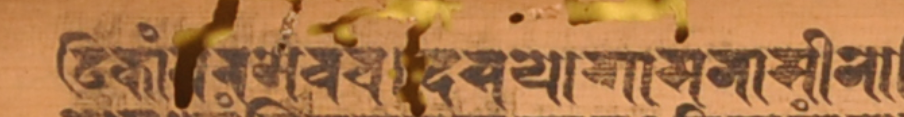
\includegraphics[scale=.3]{images/dasayoga_msNa.png}

[\skt{spha}]\skt{ṭikāṃ}\lk \skt{ram} [= \skt{°kāṃbaram}] 
\skt{eva ca} $|$ \skt{daśayogāsanāsīno}

\msL\ (\fol381v) gives:

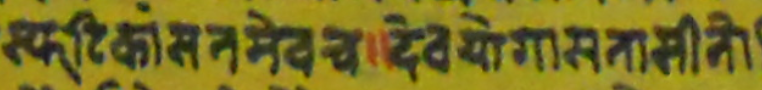
\includegraphics[scale=.3]{images/dasayoga_msL.png}

\skt{sphaṭikāṃsatam eva ca $||$ devayogāsanāsīto}
\end{quote}

\noindent
supplying \skt{sa} for the lost syllable and misreading the 
damaged \skt{da} as \skt{de} and the \skt{śa} as \skt{va}.

Here \msNa\ (\fol39v) reads:

\begin{quote}
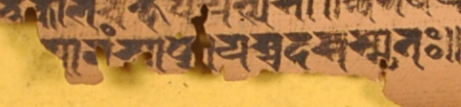
\includegraphics[scale=.5]{images/japoyoga_msNa.png}

[\skt{japo yogas tapo}] \skt{dhyānaṃ svādhyāyaś ca daśa smṛtaḥ} 

with \textit{dhyā} and \textit{svā} damaged;

\msL\ (\fol381r) cannot read the bit that 
is completely lost, and it misreads 
the damaged \skt{dhyānaṃ} as \skt{dhānaṃ}, \skt{svādhyā} as \skt{sādhu}:
\smallskip

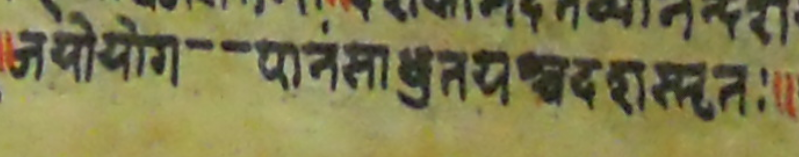
\includegraphics[scale=.3]{images/japoyoga_msL.png}
\end{quote}

\noindent
In the next example, the text is supposed to read
\skt{kare gṛhya tapodhanam~| 
tataḥ so 'ntarhitas{ }tatra tenaiva}. 


\begin{quote}
\msNa\ (\fol39r) gives:

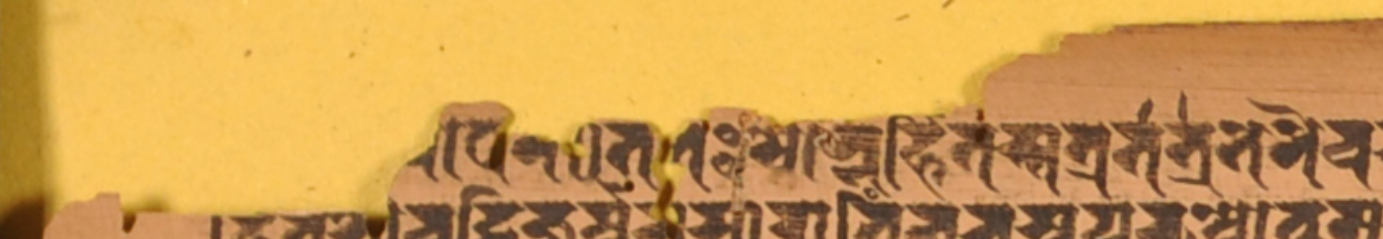
\includegraphics[scale=.21]{images/hitas_msNa.png}

[\skt{kare}] \skt{\lac\ dha\uncl{na tataḥ so 'ntar}hitas tatra tenaiva}

\msL\ (\fol380r) gives:

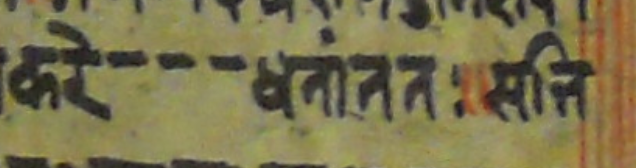
\includegraphics[scale=.3]{images/hitas01_msL.png}
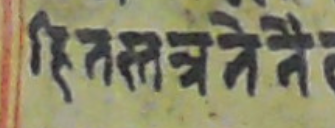
\includegraphics[scale=.3]{images/hitas02_msL.png}

\skt{kare \lac\ dhatāṃ tataḥ $||$ sati hitas tatra tenaiva}
\end{quote}

\noindent
trying to make sense of the fragments. The examples above
suggest that \msL\ was copied directly from \msNa\
when the damage had already been done to \msNa. For this reason,
I have not collated its readings for \VSS\ chapters 1--12.


\medskip


%1) Śivadharmaśāstra, %(serial no. 634), fols.~1v--63r; 
%2) Śivadharmottara, %  (s. no. 635) fols.~64r--143v; 
%3) Śivadharmasaṃgraha, % (s. no. 633), fols.~144r--217v;
%4) Umāmaheśvarasaṃvāda, % (s. no. 652), fols.~218v-- 263v; 
%5) Śivopaniṣad, %(s. no. 636), fols.~264r--297v; 
%6) Uttarottaramahāsaṃvāda, % (s. no. 654), fols.~298r--324r;
%7) Vṛṣasārasaṃgraha, % (s. no. 657), fols.~325r--390r;
%8) Dharmaputrikā. % (s. no. 608), fols.~391r--406r.





\hide{
**** Kesar 537 (NGMPP C 107/7). Paper, dated to NS 803 (1682--83 CE),
174 folios. Contents: Śivadharmasaṃgraha (fols.~89r--133v);
Umāmaheśvarasaṃvāda (fols.~134r--163v); Śivopaniṣad (fols. 164r--181r);
Uttarottaramahāsaṃvāda (fols.~182r--206v); Vṛṣasārasaṃgraha
(fols.~207r--251v); Dharmaputrikā (fols. 252r--262v).

**** Kesar 597 (NGMPP C 57/5). Paper, dated to NS 863 (1742--43 CE), 257
folios. Contents: Śivadharmaśāstra (fols.~1v--41v); Śivadharmottara
(fols.~42v--92r); Śivadharmasaṃgraha (fols. 93v--138v);
Umāmaheśvarasaṃvāda (fols.~139v-- 170v); Śivopaniṣad (fols.~171v--188r);
Uttarottaramahāsaṃvāda (fols.~189v-- 213r); Vṛṣasārasaṃgraha
(fols.~214v--257r).

-- NAK 4--2537 (NGMPP B 219/3). Paper, 339 folios. Contents:
Śivadharmaśāstra (fols.~1v--58r); Śivadharmottara (fols.~59v--123v);
Śivadharmasaṃgraha (fols.~124v--161v); Umāmaheśvarasaṃvāda (fols.
162v--238v); Vṛṣasārasaṃgraha (fols.~239v--338v). GOTIT

-- NAK 4--93 (NGMPP A 1341/6). Paper, 82 folios. Contents:
Śivadharmasaṃgraha (fols.~91r¤--135v); Vṛṣasārasaṃgraha
(fols.~204r¤--243v). GOTIT

-- NAK 4--1604 (NGMPP A 1365/3). Paper, 90 folios. Contents: Śivopaniṣad
(fols.~166v--184r); Uttarottaramahāsaṃvāda (fols.~185v--210r);
Vṛṣasārasaṃgraha (fols.~211v--255r). For a description of this
manuscript, see the record in the NGMCP online catalogue:
\textless{}http://catalogue.ngmcp.uni-hamburg.de/wiki
/A\_1365-3(1)\_Śivopaniṣad\textgreater{} ASK*}

\medskip


\medskip
\subsection{Naraharinath's edition}

\msdescr{(N)\Ed}{Ed}
Much has been said of Yogi Naraharinath's pioneering
but problematic edition (the \emph{editio princeps}) 
of the Śivadharma corpus 
(\mycite{NaraharinathSivadharma}).%
			\footnote{See, e.g.,
\mycitep{DeSiminiGods2016}{66, n.\ 190};
\citeyear{DeSiminiLachmann2017}, 542,
\mycitep{BisschopUniversal}{58--59}, and
\mycitep{SaivaUtopia}{55}.}
My impression of the text of the \VSS\ in 
Naraharinath's edition (pp.~580--678) is that its quality is
considerably inferior to those of the other texts of the corpus.
It may or may not be Naraharinath's fault; 
others must have been involved in the process of transcription, and the number and nature of the innumerable mistakes all over the text may also suggest a general problem with the typesetting process. In addition to this, it is now 
gradually becoming clearer and clearer that
Naraharinath must have used late paper MSS, and
some of the oddities in his text and some of the
alterations that are difficult to explain come in fact
therefrom. See the description of \msPaperA\ and
\msPaperC\ above.
In spite of all the noise in Naraharinath's edition, it
was useful to have his text as a starting point, and it
is sometimes useful to consider his readings.
Therefore I have recorded the readings found in his
publication for all twelve chapters given in my critical edition.


\vfill
\pagebreak


\section{Editorial policies}

\begin{quote}
- orthography: deviant orth, sandhi, punctuation?
- avagrahas usually supplied but sometimes found in the MSS, not used by me for crasis (e.g. a+a=ā)
- daṇḍas: usually 4 pādas to a verse, but I have made arbitrary decisions based on sense-units 
  because none of the sources really indicate where a verse ends (||).
  
- falsifications everywhere on purpose and accidentally

- mssALL

- [supply]
\end{quote}

SDh MSS from Nepal

stemma...

